%
% defintion.tex -- MSA definition
%
% (c) 2019 Prof Dr Andreas Müller
%
\section{Definition einer Multiskalenanalyse
\label{section:skalen und vektorraeume}}
\rhead{Definition}
Wir möchten zum Ausdruck bringen, dass Funktionen in $L^2(\mathbb R)$
mit zunehmender Genauigkeit approximiert werden können durch Funktionen,
die immer mehr Einzelheiten auflösen, so wie dies in
Abbildung~\ref{haar:figure:detail} für das Haar-Wavelet illustriert wird.
Sei also $V_0\subset L^2(\mathbb R)$ ein Vektorraum von Funktionen, wobei wir
uns vorstellen, dass darin Funktionsdetails bis zur Länge eines
Einheitsintervalls aufgelöst sind.
Im Beispiel des Haar-Wavelets wäre der Raum der auf Intervallen der Länge
$1$ stückweise konstanten Funktionen ein geeigneter Raum,
der diese Intuition wiedergibt.

Wir erwarten, dass $V_0$ dazu geeignet ist, Funktionen aus $L^2(\mathbb R)$
auf eine translationsinvariante Art zu approximieren, wenigstens
für Translationen um ganze Zahlen.
Das geht aber nur, wenn mit $f\in V_0$ auch alle um ganze
Zahlen $b\in\mathbb Z$ verschobenen Funktionen $T_bf\in V_0$ sind.

Durch Skalierung von Funktionen wird es möglich werden, weitere Details
aufzulösen.
Der Vektorraum $V_j$ soll die Menge der Funktionen umfassen, die Details
bis zur Grösse $2^{-j}$ darstellen kann.
Im Haar-Wavelet-Beispiel sind das die Funktionen, die zwischen Punkten
konstant sind, die ganzzahlige Vielfache von $2^{-j}$ sind.
Je mehr Details aufgelöst werden können, desto grösser sind die
Vektorräume.
Es entsteht ein Turm
\begin{equation}
\dots
V_{-2}\subset
V_{-1}\subset
V_0\subset
V_1\subset
V_2\subset
\dots
V_j\subset
\dots
\subset L^2(\mathbb R)
\label{buch:skalen-turm}
\end{equation}
von Unterräumen von $L^2(\mathbb R)$.

Der Turm~\eqref{buch:skalen-turm} drückt noch nicht aus, dass die
Funktionen, die höhere Details wiedergeben, skalierte Versionen der
``gröberen'' Funktionen sind.
Daher wird gefordert, dass
\[
f\in V_j \quad\Rightarrow\quad D_{\frac12}f\in V_{j+1}
\qquad\text{oder}\qquad
D_{\frac12}V_j \subset V_{j+1}
\]
Dies wiederum drückt noch nicht aus, dass in $V_{j+1}$ nicht noch mehr
Details aufgelöst werden können, als mit Hilfe von skalierten Versionen der
Funktionen in $V_j$ möglich ist.
Dazu muss verlangt werden, dass
$D_{\frac12}V_j = V_{j+1}$
gilt.

Wie in Abbildung~\ref{haar:figure:detail} suggeriert,
möchten wir die zusätzlichen Details, die $V_1$ gegenüber $V_0$ auflösen kann,
in einem orthogonalen Unterraum $W_0$ von $V_1$ unterbringen.
Wir schreiben dafür $V_1 = V_0 \oplus W_0$ und meinen damit, dass
\[
V_0\cap W_0= \{0\}
\qquad\text{und}\qquad
V_0 \perp W_0
\]
\index{orthogonale Summe}
sein muss.
Dies gilt natürlich auf jeder Detailebene, es ist also
$W_{j+1} = D_{\frac12}W_j$ und $V_j\oplus W_j = V_{j+1}$.

Es wäre zu viel verlangt, dass jede Funktion in $L^2(\mathbb R)$ in
einem der Vektorräume $V_j$ liegt, denn in $L^2(\mathbb R)$ gibt
es ja einige ``ganz verrückte'' Funktionen.
Wir verlangen daher nur, dass die Abtastung detailliert genug ist, dass jede 
Funktion in $L^2(\mathbb R)$ beliebig genau durch Funktionen aus
der Vereinigung aller $V_j$ approximiert werden kann.
Dies wird durch
\[
\overline{\bigcup_{j\in Z} V_j} = L^2(\mathbb R)
\]
ausgedrückt, wobei der Querstrich den Abschluss bezeichnet, die Menge
aller Grenzwerte von Folgen in der Vereinigung der $V_j$.

Wird die Auflösung schrittweise reduziert, dann bleibt nur die Nullfunktion
übrig.
Es gibt also keine Funktionen mit Features, die beliebig weit ausgedehnt
sind im Sinne der Vektorräume $V_j$.
Man kann dies durch
\[
\bigcap_{j\in\mathbb Z} V_j = \{0\}
\]
ausdrücken.

Damit haben wir alle Elemente zusammen für die folgende formale Definition
einer Multiskalenanalyse.

\begin{definition}
Eine {\em Multiskalenanalyse} ist ein Turm
\index{Multiskalenanalyse}%
\[
\dots
V_{-2}\subset
V_{-1}\subset
V_0\subset
V_1\subset
V_2\subset
\dots
V_j\subset
\dots
\]
von Unterräumen von $L^2(\mathbb R)$ mit den folgenden Eigenschaften
\begin{enumerate}
\item Es gibt eine Funktion $\varphi\in V_0$, das sogenannte Vaterwavelet oder
die Skalierungsfunktion,
\index{Vaterwavelet}%
\index{Skalierungsfunktion}%
derart, dass die Funktionen
$T_k\varphi$ eine orthonormierte Basis von $V_0$ bilden.
\item $D_{\frac12} V_j = V_{j+1}$
\item $\displaystyle\bigcap_{j\in\mathbb Z} V_j = \{0\}$
\item $\displaystyle\overline{\bigcup_{j\in\mathbb Z} V_j} = L^2(\mathbb R)$.
\item Es gibt eine Funktion $\psi\in V_0$, das sogenannte
Mutterwavelet, derart, dass
\index{Mutterwavelet}%
die Translate $T_b\psi$ mit $b\in\mathbb Z$ den Raum $W_0$ erzeugen:
\[
W_0 = \overline{\langle T_b\psi\;|\;b\in\mathbb Z\rangle}.
\]
\end{enumerate}
Das Orthogonalkomplement von $V_j$ in $V_{j+1}$ wird mit $W_j$ bezeichnet.
\index{Orthogonalkomplement}%
\end{definition}

Im Folgenden werden wir häufig mit ganzzahligen Translaten und
Zweierpotenzskalierungen von Funktion zu tun haben, wir führen dafür
die folgende Bezeichnung ein.

\begin{definition}
Sein $\varphi\in L^2(\mathbb R)$, dann schreiben wir für $k,j\in \mathbb Z$
\[
\varphi_{j,k} = D_{2^{-j}}T_k\varphi
\]
für die um $k$ verschobene und mit $2^{-j}$ skalierte Funktion.
\end{definition}

Man beachte, dass die Reihenfolge der Operationen $T_k$ und $D_{2^{-j}}$
von der bei der stetigen Wavelettransformation verwendeten abweicht.
Auch wird von der Multiskalenanalyse nicht verlangt, dass 
die $T_b\psi$ orthogonal sein müssen.
Wir werden aber sehen, dass sich dies immer einrichten lässt.

\begin{figure}
\centering
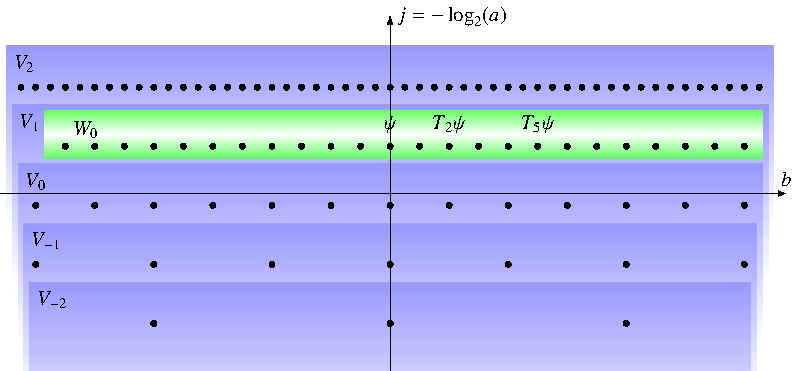
\includegraphics{chapters/6-msa/images/msa.pdf}
\caption{Hierarchie der Vektorräume $V_j$ sowie der Komplemente $W_j$
mit
$V_{j+1} = V_j \oplus = W_j$.
\label{msa:vektorraumhierarchie}}
\end{figure}

Die Funktion $\varphi$ ist enthalten in $V_0$.
Wegen $V_0\subset V_1$ ist $\varphi\in V_1$.
Da die Funktionen $\varphi_{1,k}$ eine orthonormierte Basis von $V_1$
bilden, muss es Koeffizienten $h_k$ geben derart, dass
\begin{equation}
\varphi(t) = \sum_{k\in\mathbb Z} h_k\varphi_{1,k}(t)
=
\sqrt{2}\sum_{k\in\mathbb Z}h_k\varphi(2t-k)
\label{msa:skalrel-h}
\end{equation}
gilt.

Aus der Tatsache, dass die Funktionen $\varphi_{1,k}$ eine orthonormierte
Basis von $V_1$ bilden, kann man schliessen, dass es Koeffizienten $g_k$
geben muss derart, dass
\begin{equation}
\psi(t)
=
\sum_{k\in\mathbb Z} g_k\varphi_{1,k}(t)
=
\sum_{k\in\mathbb Z}\sqrt{2}g_k \varphi(2t-k).
\label{msa:skalrel-g}
\end{equation}
A priori haben die Koeffizienten $g_k$ nichts mit den Koeffizienten $h_k$
zu tun.
Wir werden später zeigen, dass eine Multiskalenanalyse und damit
insbesondere auch die $g$-Koeffizienten vollständig durch
die $h$-Koeffizienten bestimmt sind.

\begin{beispiel}
Das Haar-Wavelet (Kapitel~\ref{chapter:haar-wavelet}) erzeugt eine
Multiskalenanalyse von $L^2(\mathbb R)$.
\end{beispiel}

